\begin{frame}{Attention Models}
  \centering
  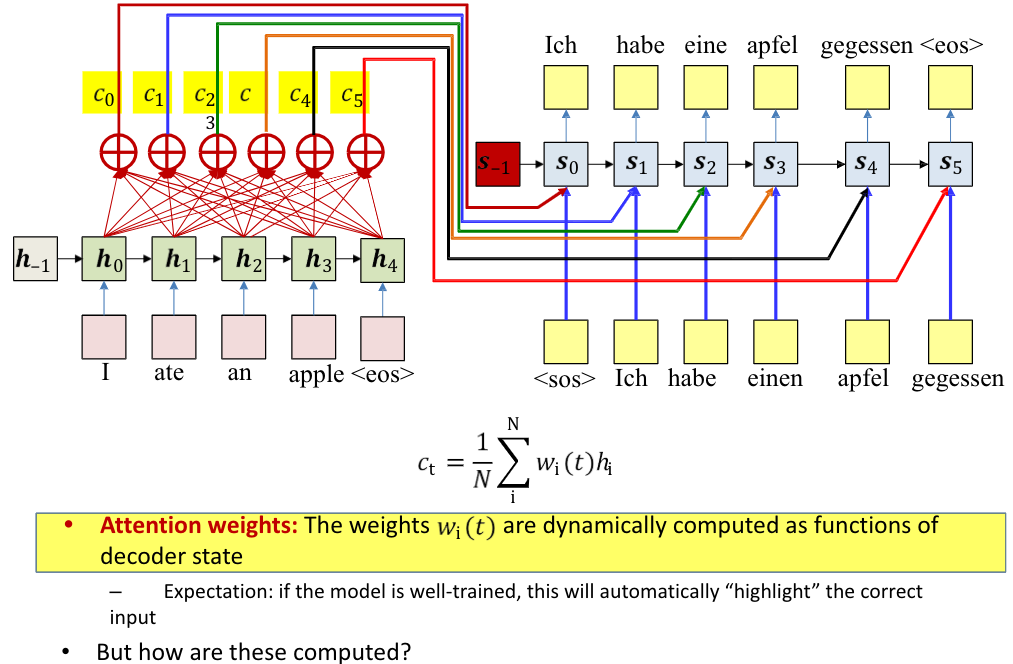
\includegraphics[width=0.5\paperwidth, height=0.5\paperheight, keepaspectratio]{assets/Lecture-5_Attention_Mechanism_Deep_Dive/pdf_page_008.png}

  % \begin{equation*}
  %   c_t = \frac{1}{N} \sum_{i=1}^N w_i(t) h_i
  % \end{equation*}
  % % \vspace{0.5em}

  % \begin{tcolorbox}[colback=yellow!20, colframe=yellow!80!black, title=Attention weights]
  %   \textbf{Attention weights:} The weights $w_i(t)$ are dynamically computed as functions of decoder state.
    
  %   % \vspace{0.25em}
  %   \begin{itemize}
  %     \item \textit{Expectation: if the model is well-trained, this will automatically ``highlight'' the correct input.}
  %   \end{itemize}
  % \end{tcolorbox}
  % % \vspace{0.5em}
  % \textbf{But how are these computed?}
\end{frame}

% slide 9
\begin{frame}{Attention weights at time $t$}
  \centering
  
\includegraphics[width=0.5\paperwidth,height=0.5\paperheight,keepaspectratio]{assets/Lecture-4_Sequence_to_Sequence_Models_Intro_to_Attention/slide_036.png}  
  \begin{itemize}
      \item The ``attention'' weights $w_i(t)$ must be computed from available information at time $t$.
      \item The primary information is $s_{t-1}$ (the state at time $t-1$).
      \item Also, the input word at time $t$, but generally not used for simplicity.
  \end{itemize}
  \begin{equation*}
      c_t = \sum_{i=1}^N w_i(t) h_i
  \end{equation*}
\end{frame}

% Slide 10
\begin{frame}{Requirement on attention weights}
  \centering
  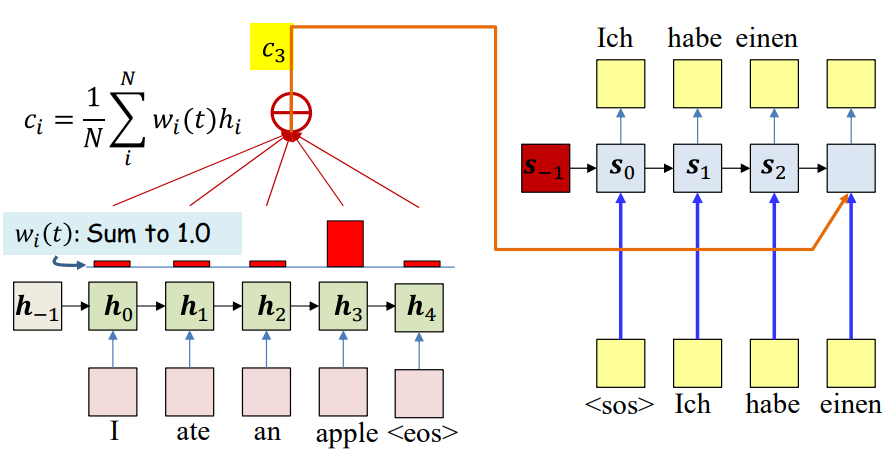
\includegraphics[width=0.5\paperwidth,height=0.5\paperheight,keepaspectratio]{assets/Lecture-4_Sequence_to_Sequence_Models_Intro_to_Attention/slide_037.png}
  \begin{itemize}
      \item The weights must be positive and sum to 1.0 (i.e., be a distribution).
      \item Ideally, they must be high for the most relevant inputs for the $i$-th output and low elsewhere.
      \item \textbf{Solution: A two step weight computation}
      \begin{itemize}
          \item First compute raw weights (which could be +ve or –ve).
          \item Then softmax them to convert them to a distribution.
      \end{itemize}
  \end{itemize}
\end{frame}

% Slide 11
\begin{frame}{Requirement on attention weights}
  \centering
  
\includegraphics[width=0.5\paperwidth,height=0.5\paperheight,keepaspectratio]{assets/Lecture-4_Sequence_to_Sequence_Models_Intro_to_Attention/slide_038.png}
\end{frame}



% Slide 12
\begin{frame}{\textcolor{green!60!black}{QUIZ}}
  \begin{itemize}
    \item[$\star$] The attention framework computes a different ``context'' vector at each output step (T/F)
      \begin{itemize}
        \item[$\blacklozenge$] True
        \item[$\blacklozenge$] False
      \end{itemize}
  \end{itemize}
\end{frame}

% Slide 13
\begin{frame}{\textcolor{green!60!black}{QUIZ}}
  \begin{itemize}
    \item[$\star$] The attention framework computes a different ``context'' vector at each output step (T/F)
    \begin{itemize}
      \item[$\blacklozenge$] \textcolor{green!60!black}{\textbf{True}}
      \item[$\blacklozenge$] False
    \end{itemize}
  \end{itemize}
\end{frame}

% Slide 14
\begin{frame}{\textcolor{green!60!black}{QUIZ}}
  \begin{itemize}
    \item[$\star$] The context vector is chosen as the hidden (encoder) representation of the input word that is assigned the highest attention weight (T/F)
      \begin{itemize}
        \item[$\blacklozenge$] True
        \item[$\blacklozenge$] False
      \end{itemize}
  \end{itemize}
\end{frame}

% Slide 15
\begin{frame}{\textcolor{green!60!black}{QUIZ}}
  \begin{itemize}
    \item[$\star$] The context vector is chosen as the hidden (encoder) representation of the input word that is assigned the highest attention weight (T/F)
    \begin{itemize}
      \item[$\blacklozenge$] \textcolor{green!60!black}{\textbf{True}}
      \item[$\blacklozenge$] False
    \end{itemize}
  \end{itemize}
\end{frame}

% Slide 16
\begin{frame}{\textcolor{green!60!black}{QUIZ}}
  \begin{itemize}
    \item[$\star$] The attention weight to any input word is a function of the hidden encoder representation of the word and the most recent decoder state (T/F)
      \begin{itemize}
        \item[$\blacklozenge$] True
        \item[$\blacklozenge$] False
      \end{itemize}
  \end{itemize}
\end{frame}

% Slide 17
\begin{frame}{\textcolor{green!60!black}{QUIZ}}
  \begin{itemize}
    \item[$\star$] The attention weight to any input word is a function of the hidden encoder representation of the word and the most recent decoder state (T/F)
    \begin{itemize}
      \item[$\blacklozenge$] \textcolor{green!60!black}{\textbf{True}}
      \item[$\blacklozenge$] False
    \end{itemize}
  \end{itemize}
\end{frame}

% Slide 18
\begin{frame}{Requirement on attention weights}
  \centering
  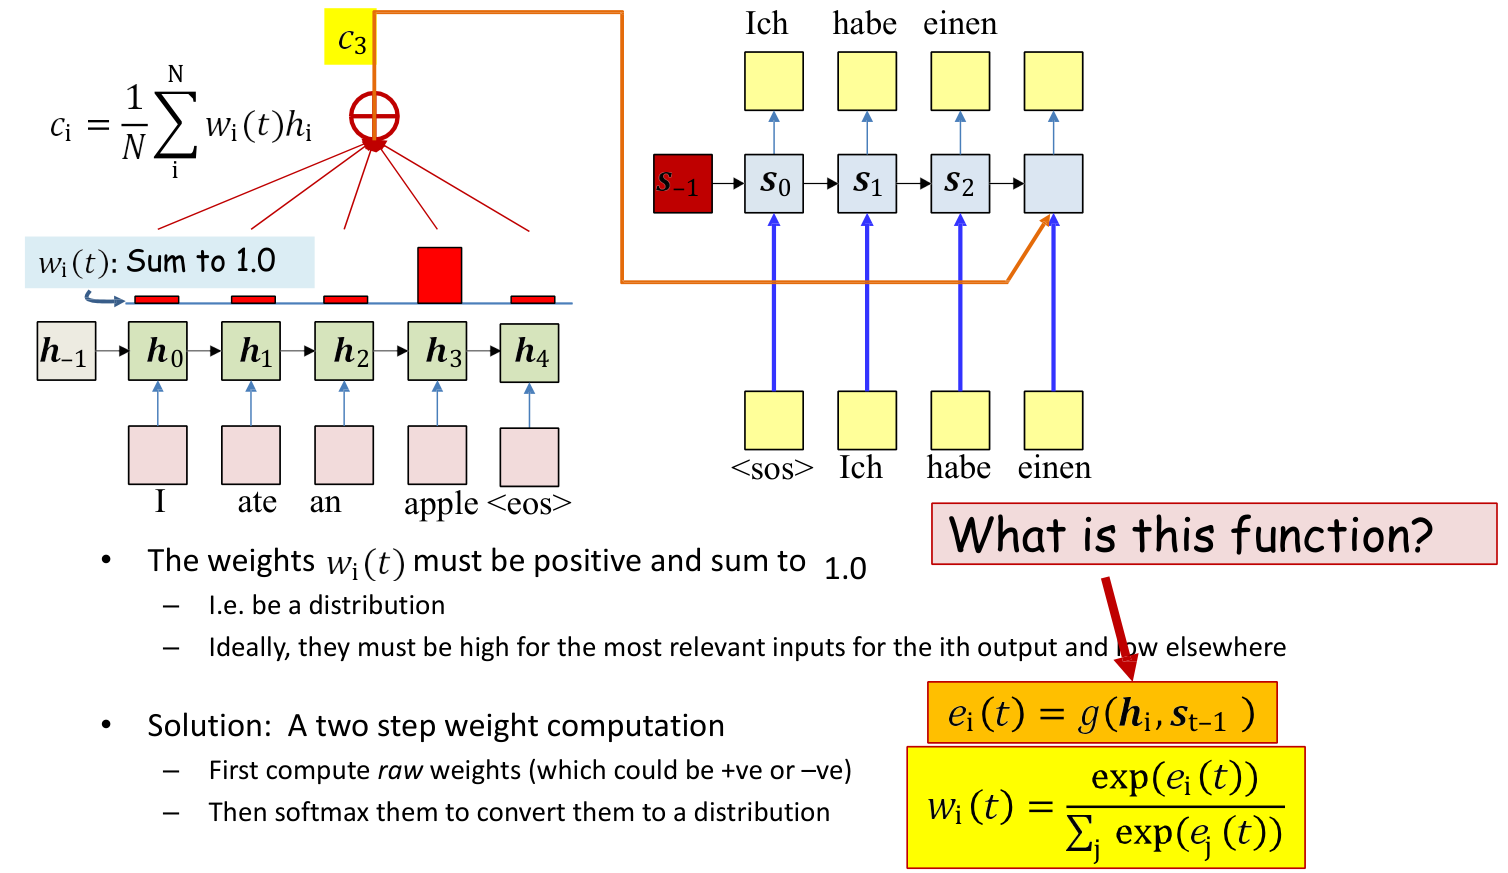
\includegraphics[width=0.5\paperwidth,height=0.5\paperheight,keepaspectratio]{assets/Lecture-4_Sequence_to_Sequence_Models_Intro_to_Attention/slide_041.png}
\end{frame}

% Slide 19
\begin{frame}{Attention weights}
  \centering
  
\includegraphics[width=0.5\paperwidth,height=0.5\paperheight,keepaspectratio]{assets/Lecture-4_Sequence_to_Sequence_Models_Intro_to_Attention/slide_042.png}
\end{frame}

% Slide 20
\begin{frame}{Attention weights}
  \centering
  
\includegraphics[width=0.5\paperwidth,height=0.5\paperheight,keepaspectratio]{assets/Lecture-4_Sequence_to_Sequence_Models_Intro_to_Attention/slide_043.png}
\end{frame}
